

% % % % % % % % % % % % % % % % % % % % % % % %


\documentclass[10pt,letterpaper]{article}
%\usepackage[top=0.85in,left=1.25in,footskip=0.75in]{geometry}




% amsmath and amssymb packages, useful for mathematical formulas and symbols
\usepackage{amsmath,amssymb}

% Use adjustwidth environment to exceed column width (see example table in text)
\usepackage{changepage}

% Use Unicode characters when possible
\usepackage[utf8x]{inputenc}

\usepackage{url}

% textcomp package and marvosym package for additional characters
\usepackage{textcomp,marvosym}

% cite package, to clean up citations in the main text. Do not remove.
\usepackage{cite}

% Use nameref to cite supporting information files (see Supporting Information section for more info)
%\usepackage{nameref,hyperref}

% line numbers
\usepackage{lineno}
\linenumbers

% ligatures disabled
\usepackage{microtype}
\DisableLigatures[f]{encoding = *, family = * }

% color can be used to apply background shading to table cells only
\usepackage[table]{xcolor}

% array package and thick rules for tables
\usepackage{array}

% create "+" rule type for thick vertical lines
\newcolumntype{+}{!{\vrule width 2pt}}

% create \thickcline for thick horizontal lines of variable length
\newlength\savedwidth
\newcommand\thickcline[1]{%
  \noalign{\global\savedwidth\arrayrulewidth\global\arrayrulewidth 2pt}%
  \cline{#1}%
  \noalign{\vskip\arrayrulewidth}%
  \noalign{\global\arrayrulewidth\savedwidth}%
}

% \thickhline command for thick horizontal lines that span the table
\newcommand\thickhline{\noalign{\global\savedwidth\arrayrulewidth\global\arrayrulewidth 2pt}%
\hline
\noalign{\global\arrayrulewidth\savedwidth}}

% Text layout
%\raggedright
%\setlength{\parindent}{0.5cm}
%\textwidth 5.25in 
%\textheight 8.75in

% Bold the 'Figure #' in the caption and separate it from the title/caption with a period
% Captions will be left justified
\usepackage[aboveskip=1pt,labelfont=bf,labelsep=period,justification=raggedright,singlelinecheck=off]{caption}
\renewcommand{\figurename}{Fig}


%tikz packages for drawing grammar trees
\usepackage{tikz}
\usepackage{tikz-qtree}
\usetikzlibrary{positioning}

% Use the PLoS provided BiBTeX style
%\bibliographystyle{plos2015}
%\usepackage{apacite}
%\bibliographystyle{apacite}
\bibliographystyle{abbrv}


%\usepackage[
%    backend=biber,
%    style=alphabetic,
%    citestyle=authoryear
%]{biblatex}

%some bibliography styles have a \citet mode which writes 
%Feckham et al (1953) instead of (Feckham et al, 1953) 
%plos2015 doesn't have this so this command replaces 
%\citet with \cite, 
%we can comment this out if we change to a 
%\citet supporting style.

\newcommand{\citet}[1]{\cite{#1}}

% Remove brackets from numbering in List of References
%\makeatletter
%\renewcommand{\@biblabel}[1]{\quad#1.}
%\makeatother

% Leave date blank
\date{}

%% Include all macros below

\newcommand{\lorem}{{\bf LOREM}}
\newcommand{\ipsum}{{\bf IPSUM}}

%% END MACROS SECTION


\begin{document}
\vspace*{0.2in}

% Title must be 250 characters or less.
\begin{flushleft}
{\Large
\textbf\newline{Grammar, lexical category and the neural processing of phrases} 
}
\newline
% Insert author names, affiliations and corresponding author email (do not include titles, positions, or degrees).
\\
Amelia Burroughs\textsuperscript{1*},
Nina Kazanina\textsuperscript{2,3},
Conor Houghton\textsuperscript{1}
\\
\bigskip
\textsuperscript{1}Department of Computer Science, University of Bristol, UK\\
\textsuperscript{2}School of Psychological Science, University of Bristol, UK\\
\textsuperscript{3}Centre for Cognition and Decision making, Institute for Cognitive Neuroscience, National Research University Higher School of Economics, Russian Federation
\\
\bigskip

% Use the asterisk to denote corresponding authorship and provide email address in note below.
* amelia.burroughs@bristol.ac.uk

\end{flushleft}


\section*{Acknowledgements}
CJH and AB acknowledge support through a James S. McDonnell Foundation Scholar Award in Cognition (JSMF \#220020239). NK acknowledges the support by the HSE Basic Research Program and the Russian Academic Excellence Project '5-100' 



% Please keep the abstract below 300 words
\section*{Abstract}

The interlocking roles of lexical, syntactic and semantic processing in language comprehension has been the subject of longstanding debate. Recently, the cortical response to a frequency-tagged linguistic stimulus has been shown to track the rate of phrase and sentence, as well as syllable, presentation. This could be interpreted as evidence for the hierarchical processing of speech, or as a response to the repetition of lexical category. To examine the extent to which hierarchical structure plays a role in language processing we record EEG from human participants as they listen to isochronous streams of monosyllabic words. Comparing responses to sequences in which lexical category is strictly alternating and chosen such that two-word phrases can be grammatically constructed --- ``cold food loud room'' --- or is absent --- ``rough give ill tell'' --- showed cortical entrainment at the two-word phrase rate was only present in the grammatical condition. Thus, lexical category repetition alone does not yield entertainment at higher level than a word. On the other hand, no cortical entrainment was found for the mixed-phrase condition that contained two-word phrases but no lexical category repetition --- ``that word send less'' --- as one would expect if the measured entrainment reflected purely abstract hierarchical syntactic units. Our results support a model in which word-level lexical category information is required to build larger units.


\section*{Introduction}

The ability of the human brain to rapidly generate meaning from an incoming stream of words is an impressive feat. The role played by hierarchical syntactic structure during this processing is the subject of an ongoing debate with, on the two extremes, some arguing that full hierarchical analysis is central to sentence comprehension \citet{Chomsky1995,BerwickEtAl2013, EveraertEtAl2015}, while others claim that hierarchical representations are not always required \cite{FrankEtAl2012, FrankBod2011, FrankYang2018, FrankChristiansen2018}.

According to the hierarchical account of language, comprehension is underpinned by the brain's ability to abstract over a number of linguistic levels, such as lexical categories such as verb, noun, adjective, and  phrases (verb phrases, noun phrases and so on) and combine them hierarchically according to a set of grammatical principles. In this view language users parse an incoming sequence of words into a nested tree-like structure that details taxonomy-like relationships between syntactic constituents and enables sentence comprehension (Fig.~\ref{fig:freq_tree}). 

\begin{figure}[tb]
\begin{center}
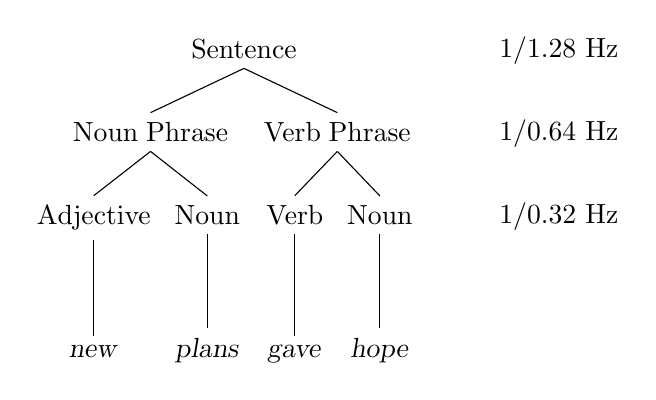
\begin{tikzpicture}
\tikzset{every tree node/.style={align=center,anchor=base}}
\tikzset{level 5+/.style={level distance=2\baselineskip}}
\tikzset{frontier/.style={distance from root=9\baselineskip}}
\Tree
    [.Sentence     
      [.Noun\;Phrase
        [.Adjective {\textsl{new}} ]
        [.Noun  {\textsl{plans}} ]
      ]
      [.Verb\;Phrase 
        [.Verb {\textsl{gave}} ]
        [.Noun {\textsl{hope}} ]
      ]
    ]
 \node at (4,0.1) {1/1.28 Hz};
 \node at (4,-0.95) {1/0.64 Hz};
 \node at (4,-2.0) {1/0.32 Hz};
\end{tikzpicture}
\end{center}
\caption{Demonstration of a syntactic tree for an example sentence from \cite{DingEtAl2016, DingEtAl2017}. The sentence is composed of a noun phrase and a verb phrase, each consisting of two words presented at a rate of 1/0.32 Hz.  The sentence is described using a hierarchical tree that splits the sentence first into a noun phrase and a verb phrase and then into words. This is a particularly simple tree, more complex trees may have more branches and not all words will be the same distance from the sentence root. This simple structure is convenient for frequency tagging and the different frequencies corresponding to the three levels of the tree; sentence, phrase and word, have been marked here. Our own experiments employed an even simpler structure with only phrases and words.}
\label{fig:freq_tree}
\end{figure}


However, it has also been suggested that the brain could rely on simpler, potentially more generic, strategies underpinned by statistical processing of linguistic representations. In line with this, recent work \cite{FrankYang2018} has shown that a model solely based on distributional word semantics is sufficient to predict the response observed in \cite{DingEtAl2016, DingEtAl2017}. In this model the distributional word semantics are represented by skipgram-word2vec vectors \cite{MikolovEtAl2013,Bojanowski2017}. In skipgram, word2vec vectors are calculated by training a simple linear neural network with one hidden layer; the input and output layers both correspond to words and the network is trained on the task of predicting, from a given one-hot input word, the unordered list of words that occur in proximity to it in text. The components of the word2vec vector for a given word are the weights feeding forwards from the word to the hidden layer. Words that are likely to occur in a similar context have similar representations in the hidden layer and hence are associated with similar word2vec vectors. To a striking degree these high-dimensional vectors have specific directions that serve, at least locally, to represent specific concepts, so that, for example, the same direction that leads from ``big'' to ``biggest'' leads from ``small'' to ``smallest'' \cite{MikolovEtAl2013b, MikolovEtAl2013c}. In \citet{FrankYang2018} fictive EEG signals representing experimental trials are constructed from the word2vec vectors for each stimulus. For each trial 320 copies of the vector for each word in the trial are lined up side-by-side forming the columns of a matrix; each column representing 1 ms of the stimulus. The rows of this matrix is then treated as a EEG and this fictive signal is analysed in the same way as the real EEG signal is and the ITPC averaged over the result for each row, much as we average over individual electrodes. This simulated EEG signal demonstrates the same entrainment to words, phrases and sentences as the real signal. Since the high-dimensional word2vec vectors represent single words only and do not explicitly encode information about word sequences, this demonstrates that semantic relationships that can be deduced from a text corpus are enough to explain the ITPC peaks seen in the real experiment, without any need to invoke the hierarchical structure of the sentence.

The current study aims to elucidate the importance of hierarchical structure during language processing using EEG. We recorded neural activity from 20 participants while they listened to streams of two-word sequences from four different conditions:
\begin{enumerate}
    \item[AN:] repetition of adjective-noun sequences, 
    \item[AV:] repetition of adjective-verb sequences, 
    \item[MP:] repetition of grammatical two-word phrases with varying lexical categories, 
    \item [RR:] random word order; no phrases possible.
    \end{enumerate}
    In the AN and AV conditions, lexical categories occurred at a regular rate, i.e. adjectives, nouns or verbs were repeated every other word. However the stream could only be parsed into grammatical phrases in the AN condition, (for example \underline{cold food} \underline{loud room} \underline{tall girl}; underlining indicates grammatical phrases). In the AV condition, no such grammatical phrases could be formed, e.g. (rough give ill tell thin chew). In the MP condition, grammatical two-word phrases could be formed, but lexical category occurred with no regularity, (for example \underline{that word} \underline{send less} \underline{too loud}). According to the hierarchical account we would expect a peak in ITPC at the phrase rate in both the AN and MP conditions, but no corresponding peak in ITPC in the AV or RR condition. A sequential account of language processing that relies primarily upon word-level statistics would instead predict a peak in ITPC at the phrasal rate in both the AN and AV conditions. 

Anticipating the main results, a peak in ITPC at the phrasal rate was only observed in the current study in the AN condition and the ITPC at the phrasal rate was significantly bigger for AN than for any of the other conditions, suggesting that neural entrainment cannot be explained solely by hierarchical accounts or lexical category regularity; rather, it additionally calls for higher level, syntactic representations. Our results support a language system that exploits both linear and hierarchical operations of language inputs to generate meaning. 


\section*{Results}
In each of the four conditions, the word2vec distributional semantics model yields a peak in ITPC of the simulated EEG responses at the rate of syllable presentation (1/0.32 Hz, Fig.~\ref{fig:Fig1}A-D). The model also yields a peak in ITPC at the rate of phrase presentation (1/0.64 Hz) for the AN and AV conditions (~\ref{fig:Fig1}A,B), where, respectively, the grammatical adjective-noun phrases or the ungrammatical adjective-verb sequences were repeatedly presented. As described in the Methods, the order of words making up the AN and AV trials were controlled to maximise the similarity in the distances between pairs of word vectors within trials as well as across the AN and AV conditions. As a result of this the model shows similar peaks in response to AN and AV trials even though the AN sequences make grammatical phrases whereas the AV sequences do not. The model also shows a pronounced, but lower amplitude peak in ITPC at the rate of phrase presentation during the MP condition (Fig.~\ref{fig:Fig1}C). The peak in ITPC at the rate of phrase presentation during the RR condition (Fig.~\ref{fig:Fig1}D) is significantly reduced.



 \begin{figure}[tbhp]
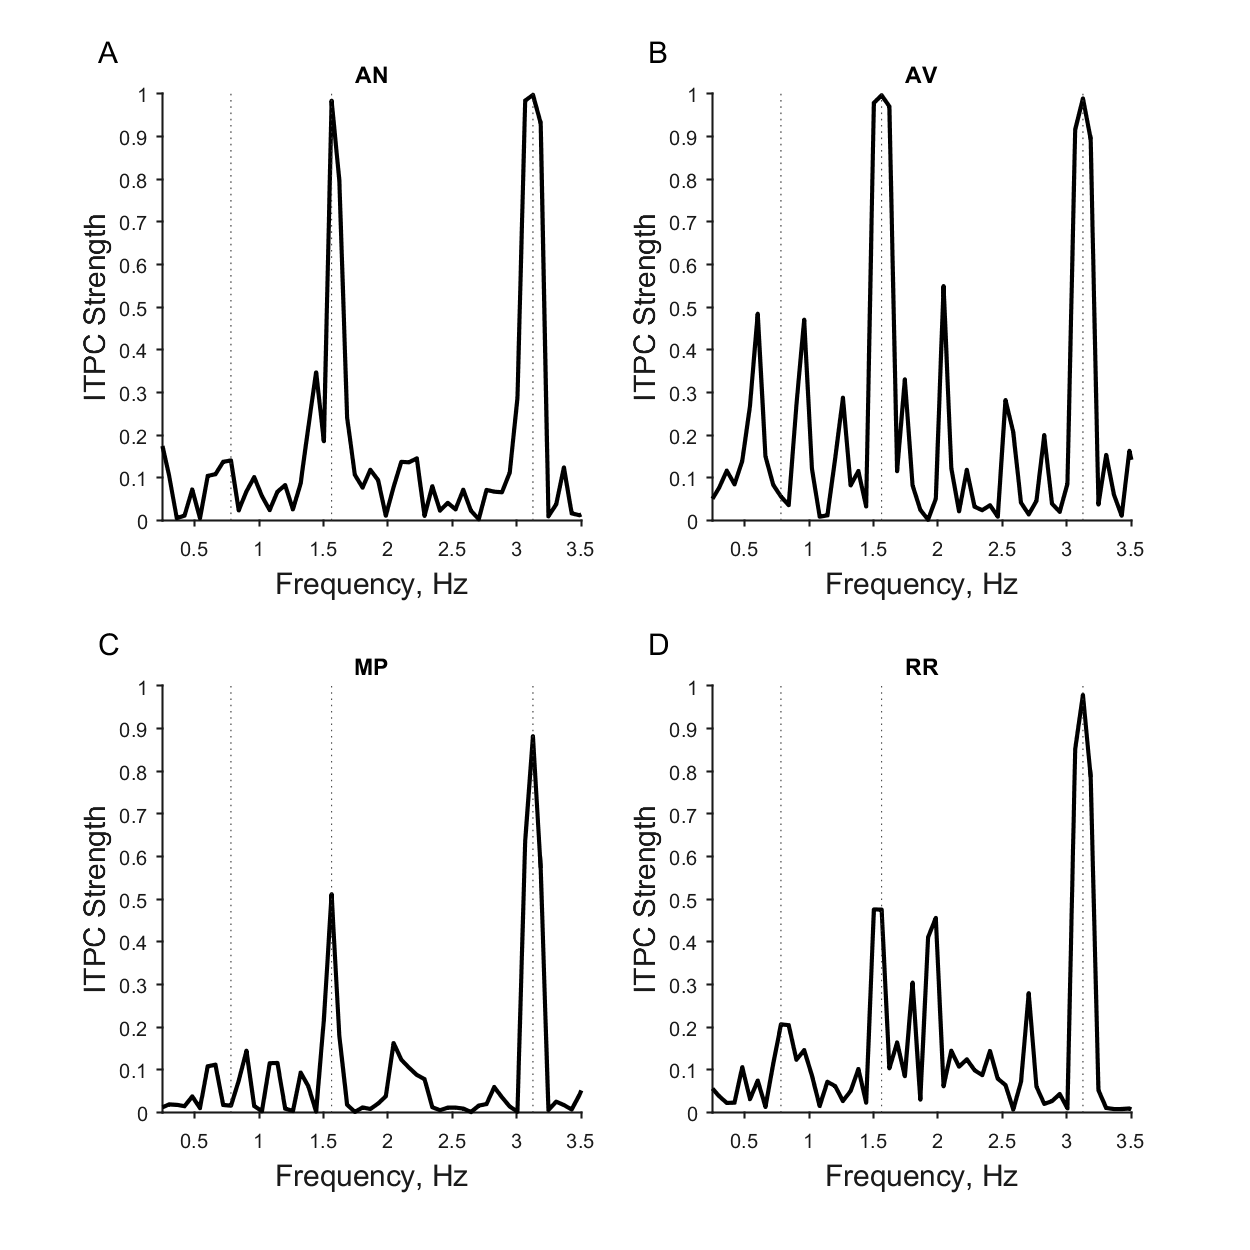
\includegraphics[width=\linewidth]{FrankFigure_exp2_phrases_12_03_2020.png}
\caption{ITPC of simulated EEG responses based on word2vec distributional semantics model predictions for the four conditions. The model yields peaks in ITPC at the rate of syllable presentation (1/0.32 Hz) in each of the four conditions (AN, AV, MP, RR). A maximal peak in ITPC at the rate at which phrases are presented (1/0.64 Hz) is seen for both the AN condition (A) where two-word sequences are grammatically well-formed and consist of repetitive lexical category information, and the AV (B) condition where two-word sequences are ungrammatical, but still have consistent lexical category information. Peaks in ITPC at the phrase rate are considerably smaller in both the MP (C) and RR (D) conditions, when compared to the peaks in ITPC at the phrase rate in the AN and AV conditions and also with the peaks in ITPC generated at the rate of syllable presentation across all conditions. Vertical gray dotted lines represent the frequency at which syllables and two-word sequences are presented.}
\label{fig:Fig1}
\end{figure}

In line with the model's prediction, EEG responses from human participants showed a significant peak in ITPC at the rate of syllable presentation (1/0.32 Hz) in all conditions tested (Fig.~\ref{fig:Fig2}A-D). However, a significant peak in ITPC at the rate of phrase presentation (1/0.64 Hz) was only observed in the grammatically well-formed AN condition (Fig.~\ref{fig:Fig2}A), which also exhibited lexical category regularity at the rate of phrases, that is, every other word came from the same lexical category. Unlike what the model predicts, in the AV condition (Fig.~\ref{fig:Fig2}B), which lacked grammatical two-word constituents but maintained lexical category regularity, no significant peak in ITPC was observed in the human EEG signal at the phrase rate (1/0.64 Hz). This peak was also absent in the MP condition (Fig.~\ref{fig:Fig2}C, grammatical two-word phrases with no lexical category regularity) and in the control RR condition (Fig.~\ref{fig:Fig2}D, word salad). A reduction in the amplitude of ITPC peaks at the phrase rate for the MP and RR conditions, when compared to the AN condition, is consistent with the model predictions.


\begin{figure}[tbhp]
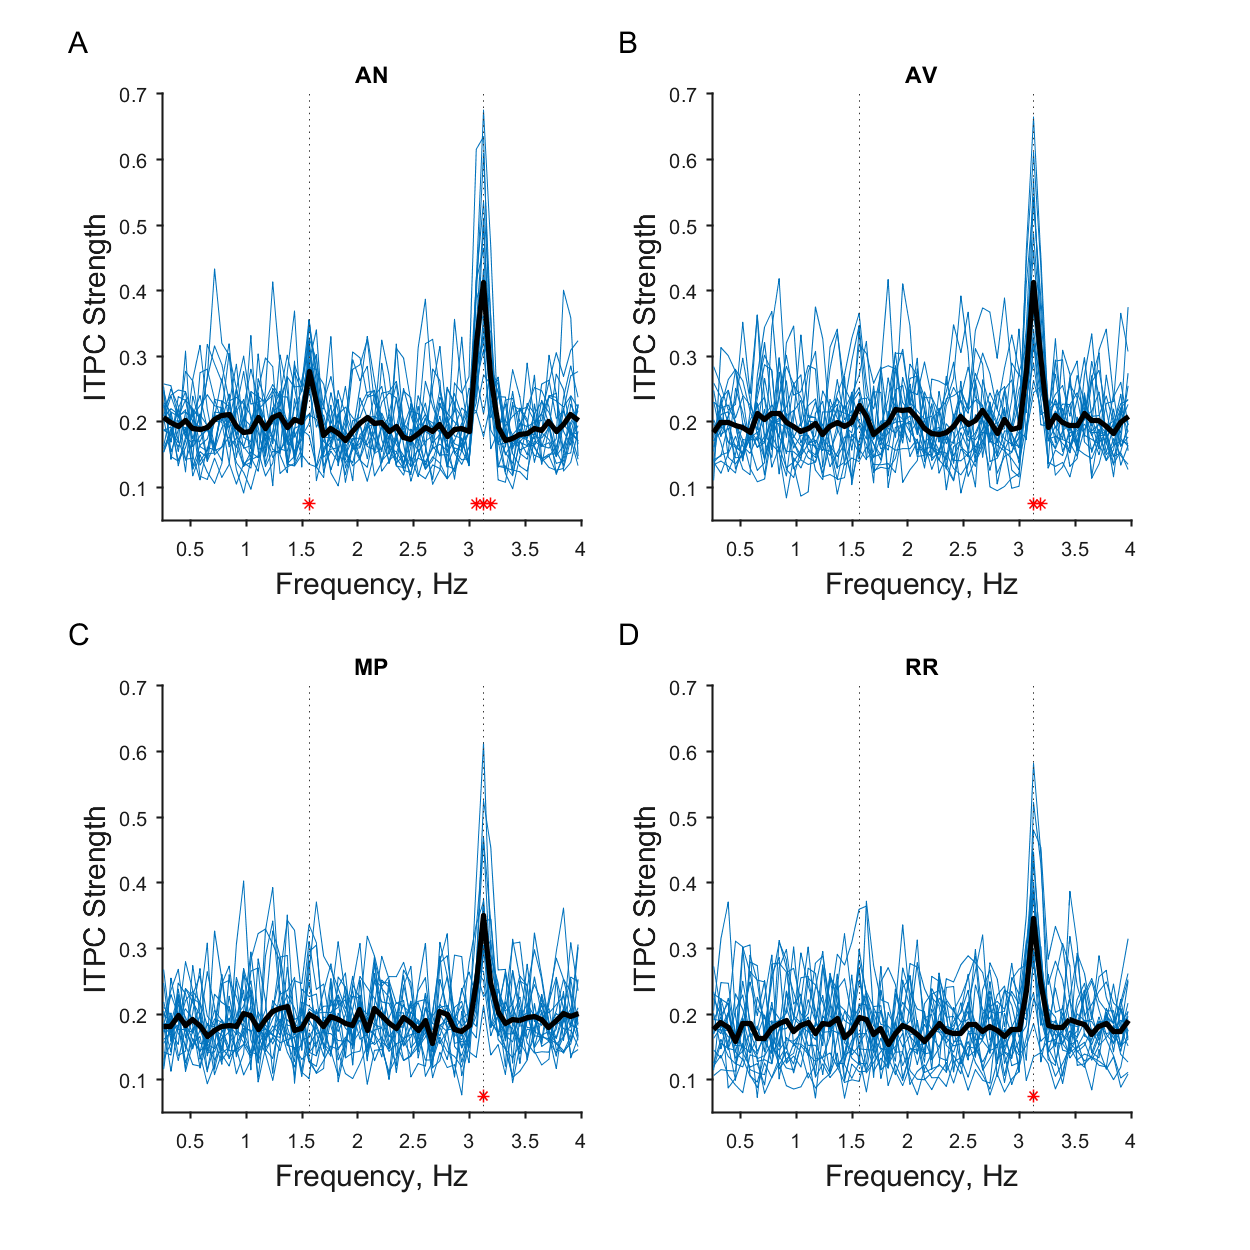
\includegraphics[width=\linewidth]{Grand_average_ITPC_for_all_phrase_conditions.png}
\caption{EEG responses recorded in human participants during presentation of trials from each of the four conditions. Statistically significant peaks in ITPC values are observed at the rate of syllable presentation (1/0.32 Hz) in each of the four conditions (AN, AV, MP, RR). A statistically significant peak in ITPC is only observed at the rate of phrase presentation (1/0.64 Hz) in the AN condition (A), where phrases are grammatically well-formed and composed of the same  lexical categories. This was not significant in any of the other three conditions (B-D). Red circles represent statistical significance *= $p<0.05$. Vertical gray dotted lines represent the frequency at which syllables and two-word sequences are presented.}
\label{fig:Fig2}
\end{figure}
\color{blue}
We next compared the ITPC values across the four conditions at the phrase and syllable rate using a one-way ANOVA. The effect of condition was significant at the phrase frequency (F(3,57)=6.05, p=0.002). Planned pairwise comparisons between ITPC amplitudes at the phrase frequency revealed that the ITPC was significantly higher in the AN condition than in each of the other three conditions (AN vs AV: p=0.024, AN vs. MP: p\<0.001, AN vs. RR: p\<0.001).The effect of condition was significant at the syllable frequency (F(3,57)=6.6, p\<0.001), however none of the planned pairwise comparisons were significant. 
\color{black}
Individual participant data: there was some participant variability and not all participants exhibited statistically significant peaks in ITPC during each of the four conditions (Fig.~\ref{fig:Fig3}). In the AN and AV conditions, statistically significant peaks at the rate of syllable presentation were observed in 18/20 participants. In both the MP and RR conditions, the peak in ITPC at the rate of syllable presentation reached significance in 17/20 participants.

When analysing the EEG responses of individual subjects at the rate of phrase presentation, a statistically significant peak was observed during the AN condition in 13/20 participants. A statistically significant peak in ITPC at the rate of phrase presentation was observed in 4/20 participants while they were listening to the AV condition, which was also the same during the MP and RR conditions. Thus the pattern observed in the grand averages can be seen in the majority of individual participants. 

\begin{figure}[tbhp]
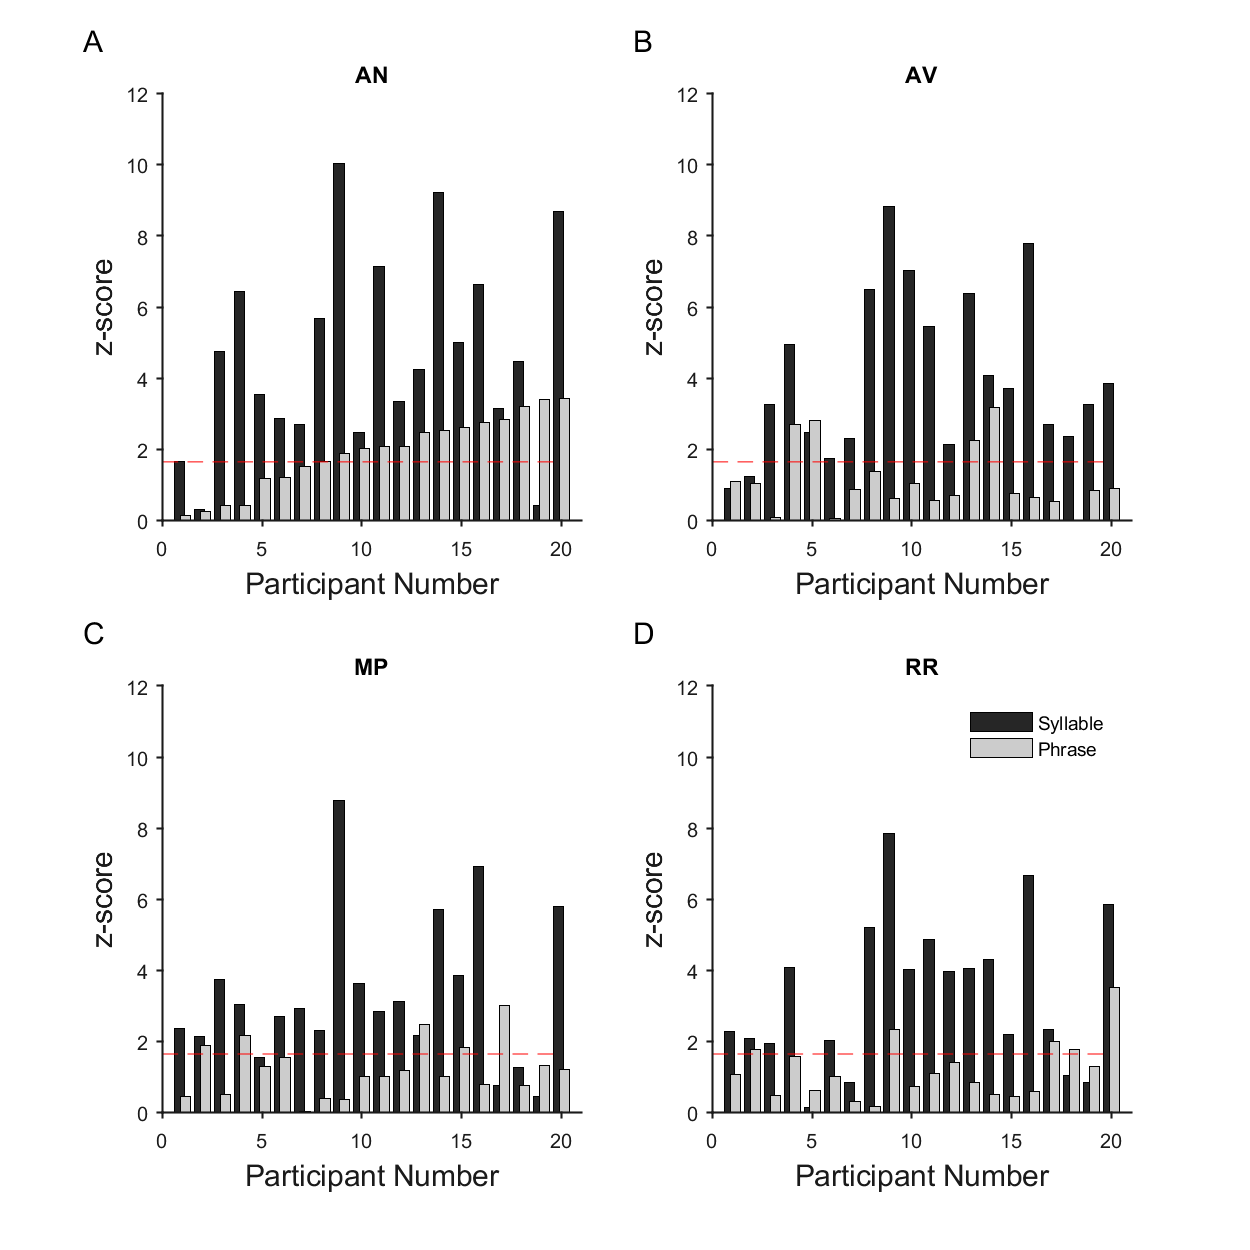
\includegraphics[width=\linewidth]{Exp2_individual_results_bar_graphs_thick.png}
\caption{Significance in ITPC at the phrase and syllable rates in individual subjects. z-scores for the ITPC at the two target frequencies: the syllable rate (black bars, 1/0.32 Hz) and phrase rate (gray bars, 1/0.64 Hz) in each of the four conditions (AN, AV, MP, RR). For each condition, z-score values of the ITPC at each frequency of interest are displayed for each of the 20 subjects. This facilitates comparison of individual subjects across target frequencies and across conditions. Participants one to 20 are ordered from left to right by the z-score of their ITPC at the phrase frequency during the AN condition (A, gray bars). Red dashed horizontal lines indicate the significance threshold ($p<0.05$, $z>1.96$) and so any z-score that is above this line represents a  ITPC that is significantly higher than chance level.}
\label{fig:Fig3}
\end{figure}


\section*{Discussion}


The current study investigated whether, and to what extent, syntactic structure is automatically utilised by the brain during language comprehension, over and above processing at the lexical level. It was found that repetitive presentation of grammatically well-formed, two-word adjective-noun phrases yields a peak in ITPC at the rate of phrase presentation, but that repetitive presentation of two-word adjective-verb sequences that cannot be combined into a phrase does not yield such a peak. The amplitude of this peak, as well as the syllable peak in response to single words, is consistent with previous findings \citet{DingEtAl2017}. This provides support for a syntactic operation that enables combining of words into higher-level syntactic units and suggests that the processing of linguistic input involves levels of abstraction beyond word-level lexical-category information. The finding supports classical syntax-based approaches to language \citet{BerwickEtAl2013,EveraertEtAl2015,Chomsky1995}. It is also generally compatible with the proposal that higher-level chunking of smaller language units occurs during language processing \citet{ChristiansenChater2016}, although the nature of what the chunks are remains somewhat unclear.

The distributional semantics model predicts a similar peak in ITPC at the rate of phrase presentation during both the AN and AV conditions. However, despite similarity in distributional vector space for the AN and AV conditions, the ITPC peak at the rate of phrase presentation was absent in the AV condition in the experimental recording. This suggests that the brain's response is not merely a function of lexical category; rather, it also reflects higher-level syntactic constituency.

However, no significant peak in ITPC at the rate of phrase presentation was found in response to the MP condition with contained repeated presentation of grammatically well-formed phrases with words from different lexical categories. While the difference we observe between the response to AN and AV sequences indicates a neural response to grammatical structure, there is no significant phrase rate response to the MP condition even though it is composed of grammatical two-word phrases. To the extent that each phrase involves combining two words into a single syntactic unit, there is a clear regularity in the MP condition at the syntactic level. Yet, this in itself is not sufficient to yield a peak in the ITPC. This might indicate that the response is not sufficiently abstract to reflect repetition of syntactic constituents independent of their lexical properties; for example, the phrases differ in the location of their head; determiner-noun phrases have the head after the modifier (``that word'') while preposition-noun phrases have their head before (``send less''). According to this interpretation, the phrase-level response found in the AN condition cannot be interpreted generally as a reflection of the Merge operation \citet{Chomsky1995} in its most general form: in both the AN and MP conditions words are pairwise merged into a phrase, but the ITPC peak only occurs in the former case.
\color{blue}
Another explanation for the lack of a significant peak in the response to the MP condition is that trials for this condition is more difficult to follow and consequently less well attended to. To investigate this we performed a behavioural study in which subjects listened to a stimulus modelled on our EEG stimulus with trials for the AN, MP and RR condition. After the last stream they were asked to indicate whether they thought the last stream was composed of two-word phrases or random words. The order of the streams were randomized, so a subject had an equal chance of being asked this question about an AN, MP or RR trial; in fact there were 33 subjects asked about an AN trial, 27 about an MP trial and 28 about an RR trial. For AN $32/33\approx 0.97$ thought the trial was made of phrases, for MP this was $24/27\approx 0.89$ and for RR it was $22/28\approx 0.79$. Thus, almost all subjects asked about an AN trial correctly that identified that is was composed of phrases, but a substantial majority of subjects asked about an RR stream incorrectly believed it was in fact composed of phrases; MP lies between the two. A Fisher Exact test shows that AN subjects were significantly ($p=0.031$) more likely to believe the stream was composed of phrases than RR subjects; the other two comparisons are not significant (AN\>MP p=0.234 and MP\>RR p=0.253). This behavioural experiment demonstrates the difficulty in parsing the stimulus as it is being listened too and does indicate that the MP trials are harder to distinguish from RR than the AN trials.
\color{black}

Certainly, any model of language comprehension must exploit linear and hierarchical structures and describe how the brain uses different types of evidence: lexical, semantic and grammatical, in deducing meaning. While these different elements had seemed difficult to reconcile, recent neural network models with a linear temporal structure are able to discover and encode hierarchical structure, see \citet{LakretzEtAl2019,Baroni2019} for example. These models are consistent with the results outlined in the current study. Here we present evidence that words are sequentially combined by the brain into phrases and that syntactical information is important for the brain's response to language; this indicates that hierarchical structure is deduced and classified, at least in part, based on syntactical information.


One issue with frequency tagging experiments, like the one presented here, is that neural mechanisms responsible for generating the ITPC in the frequency tagging paradigm are still not clear. It may be that cortical entrainment to the rate at which features of interest are presented drives the peaks in ITPC \cite{Meyer2018}, or instead it is possible that the frequency tag is driven by regularities in ERPs in response to individual words or their combination. \citet{PulvermullerEtAl2002} argues that specific networks of neurons may be sensitive to sequences of words from discrete lexical categories. In this way, local networks of neurons could learn to become sensitive to activation by a sequence of elements from different groups, for example an adjective followed by a noun, as in the AN condition presented in this study. This could explain why we only see ITPC at the phrase rate following repetitive presentation of phrases from the same syntactic class (AN). Syntactically similar adjective-noun phrases would repetitively and consistently activate the same sequence-detecting network of neurons responsible for processing adjective-noun phrases, whereas presentations of a mixture of different syntactic phrases would activate a different network of sequence-detecting neurons and thus generate an inconsistent EEG response and no peak in ITPC at the phrase rate. On the other hand there would be no sequence-detector network for ungrammatical combinations, such as adjective-verb, and these therefore fail to elicit a phrase-level response. 

In conclusion, the experiments described in the current study demonstrate that neural entrainment cannot be explained at the lexical level; rather, it additionally calls for higher-level syntactic representations. Yet, in our paradigm, frequency tagging of higher-level syntactic units emerged only in the presence of lexical category repetition, leaving open the question of how abstract syntactic representations are.


\section*{Methods}
\subsection*{Participants}

Twenty right-handed, native English speakers (12 female, mean age 25 years, range 22 - 42 years) participated in this study. Participants were screened for dyslexia and hearing impairments. All participants gave written, informed consent prior to undertaking the study and were reimbursed for their time at a rate of £10/hour. Ethical approval for our experimental procedures were obtained from the University of Bristol Faculty of Science ethics board. All methods were performed in accordance with the relevant guidelines and regulations.

\subsection*{Stimuli}

The experimental procedures were similar to those used in a recent EEG study \cite{DingEtAl2017}. Listeners were played streams of monosyllabic words in English. The words were synthesised individually using the \texttt{MacinTalk Synthesizer} (male voice \texttt{Alex}, in \texttt{Mac OS X 10.7.5}). All of the synthesised words (226 - 365 ms) were adjusted to 320 ms duration and normalised in intensity using the freely available \texttt{Praat} software \citet{Praat}.

Monosyllabic words were selected from different lexical categories, namely adjectives, nouns, verbs, pronouns, adverbs, determiners and prepositions. Words were only selected if they could be unambiguously categorised into a distinct lexical category, so, for example words such as ``drink'', ``ride'' or ``walk'' were avoided because they are ambiguous between verbs and nouns. All nouns were singular and all verbs were in the present tense.

The four experimental conditions were AN, AV, MP and RR:
\begin{enumerate}
\item Repetition of `adjective-noun' sequences (AN). 
\[
\label{eq:AN}
\text{``\underline{cold food} \underline{loud room} \underline{tall girl} \underline{bad cat} \underline{huge car} \underline{green tree} \underline{thin lamp} \underline{ill man}''}
\]
An adjective and a noun were repeated every other word. This condition contained grammatically correct two-word phrases (underlined) with the lexical category repeated every second word.

\item Repetition of `adjective-verb' sequences (AV).
\[
\label{eq:AV}
\text{``rough give ill tell thin chew hot hang green fetch small send low ask cold weep''}
\]
An adjective and a verb were repeated every other word. The word sequence in this condition preserved the repetition of lexical category but did not contain grammatically well-formed phrases.

The sequence of AN and AV words making up individual AN and AV trials was controlled so that the cosine distances between the word vectors for subsequent A and N (or V) words were similar to the distances between the word vectors for subsequent N (or V) and A words. Word vectors are described in more detail below. An initial starting word was randomly selected for each trial. Ordering words in this way minimised any consistent differences that could otherwise occur at the A to N (or V) boundaries compared to the N (or V) to A boundaries, which could introduce a peak in ITPC. The distances between the vectors of the sequences of words in AN trials were made as similar as possible to the distances between the vectors representing words in the AV trials.

\item Repetition of grammatically well-formed phrases (underlined) without repetition of lexical category information (MP).
\[
\label{eq:MP}
\text{``\underline{that word} \underline{send less} \underline{not loud} \underline{huge bird} \underline{fish cry} \underline{sheep go} \underline{the wife}''}
\]
Grammatically well-formed, two-word phrases were chosen from a pool of adjectives, nouns, verbs, pronouns, adverbs, determiners and prepositions. Phrases could take one of the following forms: `pronoun-noun', `adverb-adjective', `determiner-noun', `preposition-noun',  `verb-adverb' and these were presented in a pseudo-randomised order to avoid repetition of lexical category in adjacent phrases and to prevent grammatical phrases occurring across phrase boundaries: thus, for example, ``\underline{not loud} \underline{fish cry}'' would be excluded since ``loud fish'' is a noun phrase.

\item Pseudo-random word sequence chosen so that no phrases can be formed regularly between adjacent words.
\[
\label{eq:RR}
\text{``with chew small the his out tall old down tell soft him think at''}
\]
In this condition, words from the pool of adjectives, verbs, prepositions and determiners were randomly selected. Nouns were not included because they combine into grammatically correct phrases with words from many other lexical categories.
\end{enumerate}

A complete list of all stimuli used in the current study can be found in the Supplementary Information. In the AN and AV conditions, words were ordered such that the similarity between word2vec vectors of consecutive words in the two conditions was maximised. The average cosine distance between all adjective-verb and adjective-noun pairs was first calculated. To make one trial in the AN condition, an initial word pair was first chosen by randomly selecting a distance from the adjective-noun distance matrix that was between 0.75 and 1 (mean = 0.8). These values were hand-tuned to maximise the number of possible phrases that could be chosen whilst excluding phrases that contained dissimilar words. This gave us the first adjective-noun pair of this trial. The next adjective was then chosen as the adjective that had the closest distance to the noun from the preceding pair, but without word repetition. Similarly, the next noun was then selected as the noun that had the next closest distance from the previous adjective, but without word repetition. This was repeated for each additional word until all 52 words were chosen for the trial. This process was then repeated for each of the 25 trials with a different starting point. The same method was used to generate trials for the adjective-verb condition. This generated peaks in ITPC in the fictive EEG data that were similar for both the AN and AV conditions. In this way, we would expect that different ITPC peaks in the human EEG data are not driven by differences in the similarity of words in these two conditions (see the Results section below for an empirical confirmation).

\subsection*{Experimental Procedures}

Each trial contained a sequence of 52 monosyllabic words played back to back in a continuous stream. Trials were therefore 16.64 seconds long. In total, participants listened to 150 trials, with 25 trials for each of the four conditions here, along with two filler conditions. Blocks were made up of six trials and contained one trial from each condition plus two filler trials. Within each block, trials were presented to the participants one after the other. After each trial, participants were asked whether they heard any four word phrases, such as (either ``\underline{ask him this thing}'', ``\underline{from my old car}'' or ``\underline{sit in that tree}''). This acted as the attention trap and four-word phrases occurred in ten percent of trials. Following the button press, the next trial was played after a delay of 250 ms. At the end of each block participants were given a 10s break, with a longer 2 minute break at the halfway point. Blocks were presented in a random order that was counterbalanced across participants.

\subsection*{EEG Recording}
 
EEG signals were sampled at 1000 Hz from 32 Ag/AgCl electrodes fitted on a standard electrode layout elasticised cap using a BrainAmp DC amplifier (Brain Products GmbH). The EEG was recorded in DC mode , using a low-pass filter of 1000 Hz (fifth-order Butterworth filter with 30 dB/octave)-. FCz was used as a reference channel. The impedance of the electrodes was kept below 5 kOhms. Recordings were analysed offline using \texttt{Matlab} (Mathworks Inc.) and the \texttt{Fieldtrip} toolbox \cite{FieldTrip}. As the recordings were performed using a 32-channel system (rather than a 128-channel system as, for example, \citet{DingEtAl2017}) we did not dimension reduce our EEG signals using PCA. Eyeblink artifacts were removed using ICA. An independent component was removed if in its topography the mean power over the most frontal four channels (Fp1, Fp2, F7 and F8) was two times greater than the mean power over all other channels, as in \citet{DingEtAl2017}. As our signals of interest are in the low-frequency region, at 1/0.64 Hz (phrases), and 1/0.32 Hz (syllables), the EEG signals were filtered offline using a 25 Hz low-pass filter (sixth-order Butterworth IIR). Data were re-referenced offline to a common average reference. For each condition, individual trials (16.64s long) were epoched. Upon sound onset there is a transient EEG response and so the first four syllables (1.28 seconds) in each epoch were removed from the analysis. This meant that the overall length of the analysed part of each trial was 15.36 seconds (corresponding to 48 syllables x 0.32 s).

\subsection*{Data analysis}

After preprocessing, the EEG signal was converted into the frequency domain using the discrete Fourier transform with a frequency resolution of 0.0651 (1/15.36 Hz). The evoked power spectrum E(f) was calculated using:
\begin{equation}
\label{eq:power}
E(f)=\frac{\left|\sum{_k}X_k(f)\right|^2}{K}
\end{equation}
where $K$ is the total number of trials and $X_k(f)$ is the complex-valued Fourier coefficient of the EEG response during trial $k$. This value is a function of frequency, $f$. The evoked power reflects the power of EEG responses that are time-locked to the auditory speech input. It is the same as the power spectrum of the EEG response waveform averaged over trials.

The ITPC $R(f)$ is defined as:
\begin{equation}
\label{eq:itpc}
R(f)=\frac{\left[\sum{_k}\cos(\theta_k)\right]^2+\left[\sum{_k}\sin(\theta_k)\right]^2}{K}
\end{equation}
 where $\theta_k$ is the phase angle of each complex-valued Fourier coefficient. When analysing the inter-trial phase coherence of EEG responses in each of the four different conditions ITPC was calculated for each channel and then averaged over channels independently for each of the four conditions. 

\subsection*{Significance Testing}

Because ITPC values were averaged over channels the phase coherence cannot be easily described by a parametric distribution due to the correlation between channels. The null distribution of ITPC is therefore estimated based on the response at non-target frequencies, that is the responses at frequencies that are not harmonically related to the syllable rate \cite{DingEtAl2017}. All frequencies between 0.25 Hz and 4 Hz, other than the target frequencies +/- 2 frequency bins, were included to calculate the chance-level normalized phase coherence. To assess their significance, ITPC at target frequencies for individual participants were compared to the chance-level phase coherence. For this, the z-score at each frequency in the ITPC and the corresponding p-values were computed. A peak in ITPC was considered significant if $p < 0.05$. A one-way ANOVA was applied to the ITPC data, followed by pairwise comparisons to compare the ITPC values at the syllable and phrase frequency pairwise across conditions.


\subsection*{Simulating Word Vector ITPCs}

Word word2vec vectors were downloaded for English (\url{https://fasttext.cc/docs/en/pretrained-vectors.html}). These were calculated using a distributional semantics model that was trained on a large English corpus \citet{Bojanowski2017}. Word vector ITPC graphs were generated by first aligning word vectors representing the sequence of words in each of the trials for each of the different conditions presented to subjects in the auditory stimuli during the EEG experiment. The ITPC was then computed over these sequences of vectors as in Eq.~\ref{eq:itpc} \citet{FrankYang2018}.

\subsection*{Behavioural experiment}

For the behaviour experiment four trials were chosen for each of the AN, MP and RR conditions along with one filler trial for each of the same conditions. For each subject the trials were shuffles and two filler trials picked randomly from the four where inserted into the list at locations five and 11, making fourteen trials in all. During the experiment the trials were played in sequence and after each trial the subject was asked ``Did you hear any four-word phrases?''. After the final trial they were also asked ``In the last stream of words you hear any two-word phrases?'' and ``Write down as many things from the last stream of words you have just heard as you can remember''.

90 subjects were recruited on prolific academic (\texttt{prolific.ac}) with a £1 payment. The subjects were pre-screened by prolific academic as United Kingdom or Irish citizens living in the United Kingdom or Ireland and were asked to identify their first language; two subjects who did not answer English were excluded. No other demographic information was collected. 

The average number of words remembered from the previous trial was very low; on average subjects recalled just 3.82 words on average and often these words were not from the same most recent trial or even not represented in the experiment at all. There was also no significant difference between three conditions in the number of subjects who mistakenly answered that the previous trial contained a four-word phrase. All data and the scripts used to run the experiment are available online (\texttt{/github.com/conorhoughton/listening\textunderscore experiment\textunderscore 2020}).  

\section*{Competing Interests}
The authors declare that no competing interests exist.


\bibliography{references}

\section*{Author Contributions}
AB, NK and CJH contributed to the conception and design of the work; AB carried out the experiments, performed the analysis, prepared all figures and wrote the initial draft of the main manuscript text, CJH and NK made a significant contribution during manuscript revisions.


\section*{Figure Legends}

\subsection*{Figure 1}

Demonstration of a syntactic tree for an example sentence from \cite{DingEtAl2016, DingEtAl2017}. The sentence is composed of a noun phrase and a verb phrase, each consisting of two words presented at a rate of 1/0.32 Hz.  The sentence is described using a hierarchical tree that splits the sentence first into a noun phrase and a verb phrase and then into words. This is a particularly simple tree, more complex trees may have more branches and not all words will be the same distance from the sentence root. This simple structure is convenient for frequency tagging and the different frequencies corresponding to the three levels of the tree; sentence, phrase and word, have been marked here. Our own experiments employed an even simpler structure with only phrases and words.

\subsection*{Figure 2}
ITPC of simulated EEG responses based on word2vec distributional semantics model predictions for the four conditions. The model yields peaks in ITPC at the rate of syllable presentation (1/0.32 Hz) in each of the four conditions (AN, AV, MP, RR). A maximal peak in ITPC at the rate at which phrases are presented (1/0.64 Hz) is seen for both the AN condition (A) where two-word sequences are grammatically well-formed and consist of repetitive lexical category information, and the AV (B) condition where two-word sequences are ungrammatical, but still have consistent lexical category information. Peaks in ITPC at the phrase rate are considerably smaller in both the MP (C) and RR (D) conditions, when compared to the peaks in ITPC at the phrase rate in the AN and AV conditions and also with the peaks in ITPC generated at the rate of syllable presentation across all conditions. Vertical gray dotted lines represent the frequency at which syllables and two-word sequences are presented.

\subsection*{Figure 3}

EEG responses recorded in human participants during presentation of trials from each of the four conditions. Statistically significant peaks in ITPC values are observed at the rate of syllable presentation (1/0.32 Hz) in each of the four conditions (AN, AV, MP, RR). A statistically significant peak in ITPC is only observed at the rate of phrase presentation (1/0.64 Hz) in the AN condition (A), where phrases are grammatically well-formed and composed of the same  lexical categories. This was not significant in any of the other three conditions (B-D). Stars represent statistical significance *= $p<0.005$. Vertical gray dotted lines represent the frequency at which syllables and two-word sequences are presented.

\subsection*{Figure 4}

Significance in ITPC at the phrase and syllable rates at the individual subject level. z-scores for the ITPC at the two frequencies of interest: the syllable rate (dark gray bars, 1/0.32 Hz) and phrase rate (light gray bars, 1/0.64 Hz) in each of the four conditions (AN, AV, MP, RR). The graphs for each participant are positioned next door to one another. For each condition, z-score values of the ITPC at each frequency of interest are displayed for each of the 20 subjects. This facilitates comparison of individual subjects across both frequencies of interest and across conditions. Participants one to 20 are ordered from left to right by the significance of their ITPC at the phrase rate during the AN condition (A, light gray bars). Red dashed horizontal lines indicate the significance threshold ($p<0.005$, $z>1.96$) and so any z-score that is above this line represents a  ITPC that is significantly higher than chance level.

\end{document}

